\documentclass[12pt, a4paper]{article}
\usepackage[utf8]{inputenc}
\usepackage[makeroom]{cancel}
\usepackage{amsmath}
\usepackage{amssymb}
\usepackage{empheq}
\usepackage{xcolor}
\usepackage{graphicx} %imagens, etc
\usepackage{placeins} %sem isso suas imagens vao parar na 19-esima dimensao
\usepackage[export]{adjustbox}
\usepackage{caption} 
\usepackage{subcaption}
\usepackage{verbatim}
\usepackage{caption}
\usepackage{tabularx}
%* * * * * * * * * * * * * * * * * *%

%margens do documento
\usepackage{geometry}
\geometry
{
	a4paper     ,
	left=3.0cm  ,
 	top=3.5cm   , 
 	right=2.0cm ,
 	bottom=2.0cm
}

%indenta o primeiro parágrafo
\usepackage{indentfirst}

%endentação dos parágrafos
\setlength{\parindent}{1.25cm}

%espaço antes de cada parágrafo
\setlength{\parskip}{1em}

%espaço entre as linhas de cada parágrafo
\renewcommand{\baselinestretch}{1.2}

%troca titulo do contests
\renewcommand*\contentsname{Sumário}

%* * * * * * * * * MATH * * * * * * * * *%

%espaço vertical entre linhas dentro de \align
\setlength{\jot}{10pt}

%definição da capa
\title{Análise de Regressão Linear \\ Grupo 4}
\author{Heitor Augustaitis de Oliveira \\
        Lucas Moura de Carvalho \\
        Bruno Sergio Procopio Junior \\
        Thales Simão do Amaral Camargo \\
        Matheus Taipina Benini \\
        Bruno de Oliveira Feitosa }
\date{28/09/2020}


%inicio do documento
\begin{document}
\maketitle

\thispagestyle{empty} %remove a numeracao da capa

\begin{center}
    \vspace*{\fill}	
    São Paulo–SP\\
    2020
\end{center}

\newpage

\tableofcontents

\thispagestyle{empty}

\newpage

\section{Introdução}

\subsection{Motivação}

Este relatório tem como objetivo mostrar as análises feitas pelo grupo, utilizando a
linguagem R e a técnica de regressão linear, sobre a base de dados
\emph{summer-products-with-rating-and-performance\_2020-08}. A preparação do ambiente de
trabalho e as ferramentas empregadas serão apresentadas, assim como os comandos
utilizados para processar os dados e suas respectivas saídas.

Uma questão natural é se os produtos seguem a economia de escala, onde quanto mais se vende mais se diminui o preço dele. A relação entre as unidades vendidas e a sua nota geral pode ser usada como teste de sanidade da suposição de que quanto mais se vende mais avaliado é um item. Outra questão interessante é o comportamento do preço do varejo (do consumidor final) em relação ao preço. Por fim as colunas em relação ao vendedor foram selecionadas para adicionar variedade a análise, vendedores com notas maiores tem maior nota de produtos, menores preços?

\subsection{Preparação do ambiente}

Para as nossas análises, utilizamos a linguagem R e as ferramentas R Studio e Jupyter
Notebook. Tanto o script em R (.r) quanto o notebook (.ipynb) utilizado estão disponíveis aqui. Duas bibliotecas além do ``base" foram utilizadas, a \textbf{dplyr} que é uma coleção de ferramentas para facilitar o manuseio de objetos como \emph{data frames} e o \textbf{ggplot2} que é excelente para a criação de gráficos.

Execução dos comandos de carregamento da base dados e seleção
dos campos a serem trabalhados:

\FloatBarrier
\begin{figure}[h]
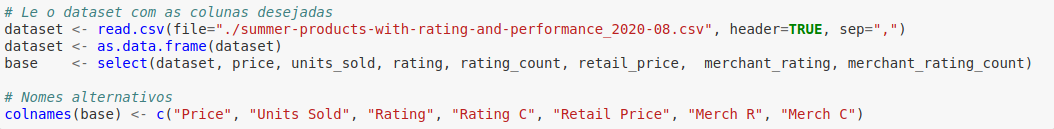
\includegraphics[scale=0.43, center]{./imgs/dataset_read.png}
\end{figure}
\FloatBarrier 

A base de dados veio sobre formato \emph{.csv} e sobre ela escolhemos sete colunas que condizem com as motivações da escolha da base, eles foram renomeadas de acordo com a tabela abaixo. \\


\begin{tabularx}{0.8\textwidth} { 
  | >{\centering\arraybackslash}X 
  | >{\centering\arraybackslash}X 
  | >{\centering\arraybackslash}X | }
 \hline
 Coluna original & Coluna Nova & Significado \\
 \hline
  price & Price & preço do item\\ \hline
  units\_sold & Units Sold & número de unidades vendidas\\ \hline
  rating & Rating & Sumário das notas dadas ao produto \\ \hline
  rating\_count & Rating C & quantidade de notas dadas ao produto \\ \hline
  retail\_price & Retail Price & preço de varejo \\ \hline
  merchant\_rating & Merch R & sumário das notas dadas ao vendedor\\ \hline
  merchant\_rating\_count & March C & quantidade das notas dadas ao vendedor\\ \hline
\end{tabularx} 
\begin{center}
	\emph{Tabela de colunas}
\end{center}

\section{Análise Inicial}

\subsection{Correlações}

A primeira análise foi feita com uma matriz de correlação das colunas, a baixo está o seu mapa de calor.

\FloatBarrier
\begin{figure}[h]
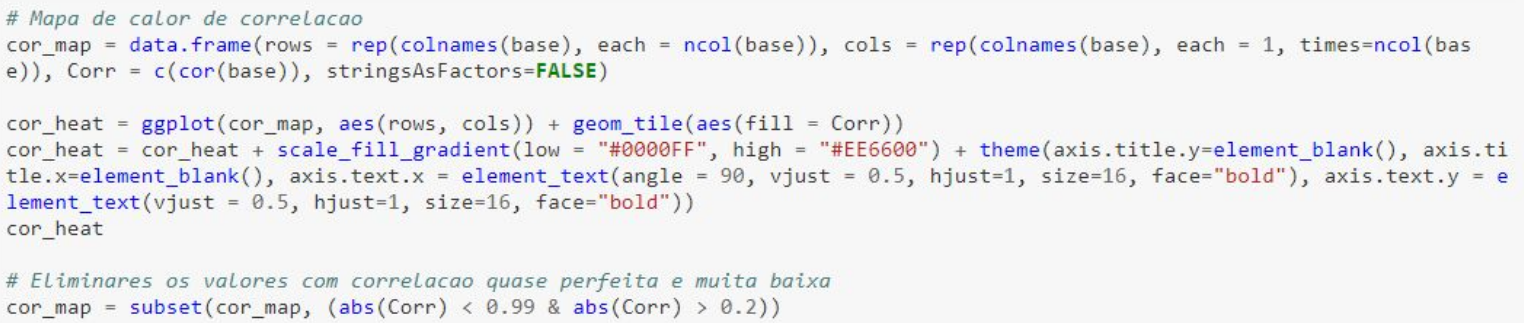
\includegraphics[scale=0.3, center]{./imgs/cod_heatmap.png}
\end{figure}
\FloatBarrier 

\FloatBarrier
\begin{figure}[h]
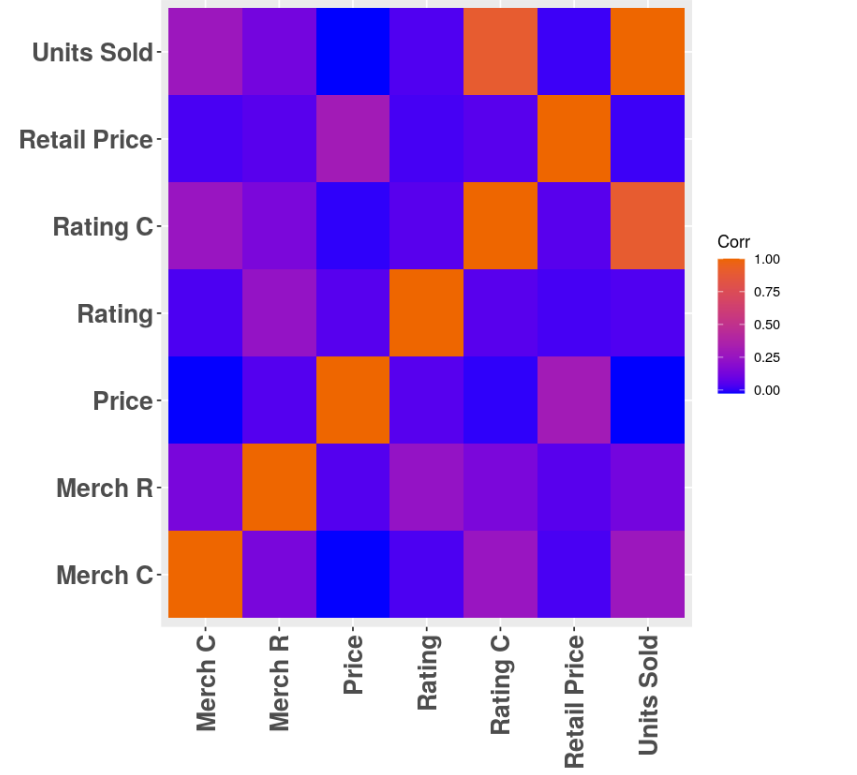
\includegraphics[scale=0.3, center]{./imgs/heatmap.png}
\caption*{Matriz de Correlação}
\end{figure}
\FloatBarrier 


Observando a matriz, nota-se uma correlação com valor alto além das identidades, que é o de Rating C com Units Sold, o que era de se esperar. Dessa matriz foram eliminados os valores com correlação menor que 0.2 já que não há linearidade aparente significante.

\subsection{Tratamento de outliers}

Para uma regressão linear, a existência de outliers pode ser especialmente nociva uma vez que as posições dos valores é levadae em consideração de maneira linear e ascendente. Nas imagens abaixo fica nítido esse problema, onde dos pontos da curva $f(x) = x$ há apenas um outlier $(18,\;30)$ na priemira (1) e $(18,\; 100)$ na segunda (2), que jogam a reta do modelo para longe dos outros pontos.\\

\FloatBarrier
\begin{figure}[h]
  \begin{subfigure}[b]{0.4\textwidth}
    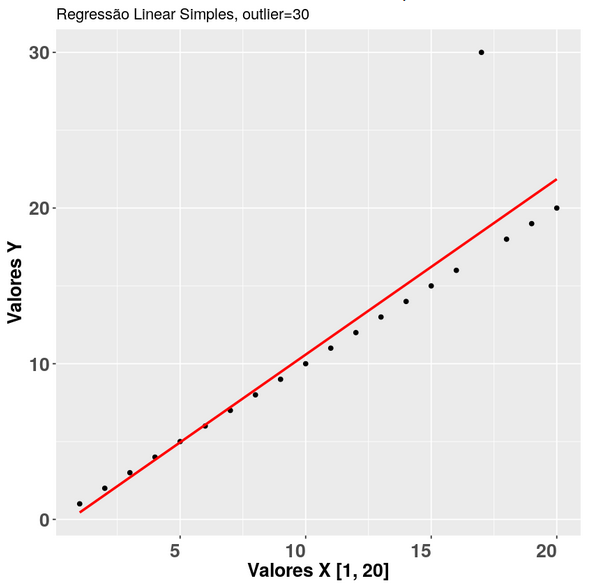
\includegraphics[scale=0.38, center]{./imgs/outlier30.png}
    \caption*{1. Regressão com outlier = 30}
    \label{fig:1}
  \end{subfigure}\hspace{1.5cm}
  \begin{subfigure}[b]{0.5\textwidth}
    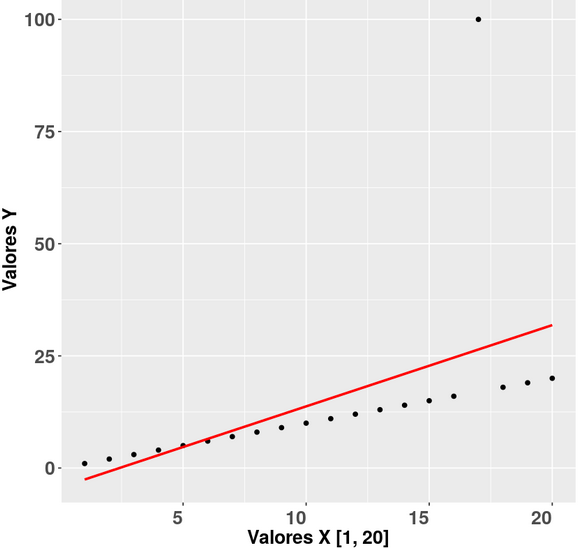
\includegraphics[scale=0.382, center]{./imgs/outlier100.png}
    \caption*{2. Regressão com outlier = 100}
    \label{fig:2}
  \end{subfigure}
\end{figure}
\FloatBarrier

Foi criada uma função que remove linhas do dataset, se baseando em uma das colunas. É calculado o intervalo interquartil e são eleminados os valores além dos limites superior e inferior.

\FloatBarrier
\begin{figure}[h]
  \begin{subfigure}[b]{0.4\textwidth}
    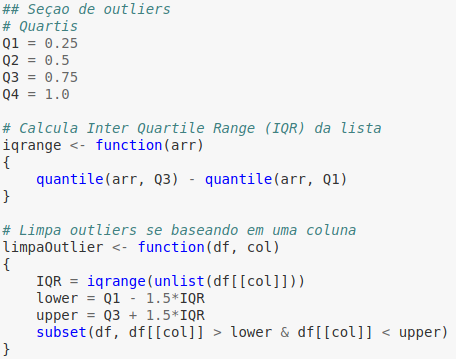
\includegraphics[scale=0.44, center]{./imgs/cod_outliers.png}
    \caption*{3. Código para outliers}
    \label{fig:1}
  \end{subfigure}\hspace{1cm}
  \begin{subfigure}[b]{0.5\textwidth}
    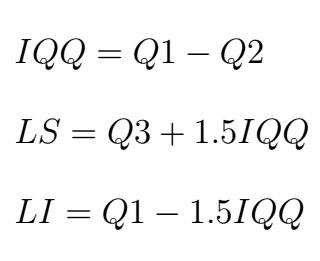
\includegraphics[scale=0.44, center]{./imgs/iqr.png}
    \caption*{4. Definições de IQQ, LS, LI}
    \label{fig:2}
  \end{subfigure}
\end{figure}
\FloatBarrier

Sobre a matriz de correlação foram aplicados os tratamentos de outliers e foram selecionados apenas os pares que sofreram um aumento na correlação.\\

\FloatBarrier
\begin{figure}[h]
	\hspace{1cm}
  \begin{subfigure}[b]{0.4\textwidth}
    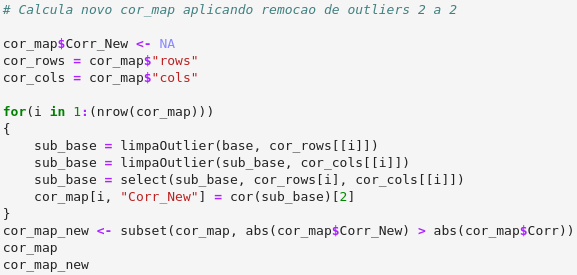
\includegraphics[scale=0.4, center]{./imgs/outlier_map.png}
    \caption*{5. Tratamento de outliers 2 a 2}
    \label{fig:1}
  \end{subfigure}\hspace{0.5cm}
  \begin{subfigure}[b]{0.5\textwidth}
    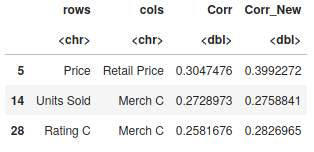
\includegraphics[scale=0.6, center]{./imgs/cor_new.png}
    \caption*{6. Resultados}
    \label{fig:2}
  \end{subfigure}
\end{figure}
\FloatBarrier

\begin{comment}
\FloatBarrier
\begin{figure}[h]
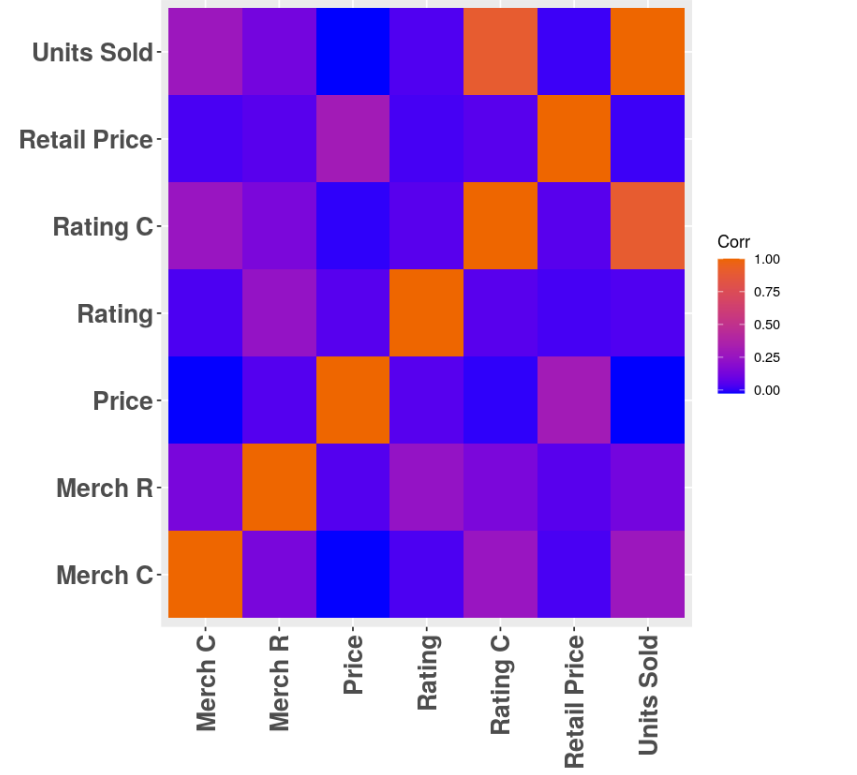
\includegraphics[scale=0.3, center]{./imgs/heatmap.png}
\caption*{Figura 3: Matriz de Correlação}
\end{figure}
\FloatBarrier 
\end{comment}

\section{Análise de Regressão}

Baseando-se na alta correlação encontrada entre Rating Count e Units Sold, foi feita a
análise de regressão linear para essas duas variáveis, sendo Units Sold a variável
dependente e Rating Count a variável independente.

É possível observar alguns resultados positivos da análise, como o valor 0.809 para o $R^{2}$ e o baixo valor para p-value, mostrando que a variável possui significância estatística para o modelo. 


\FloatBarrier
\begin{figure}[h]
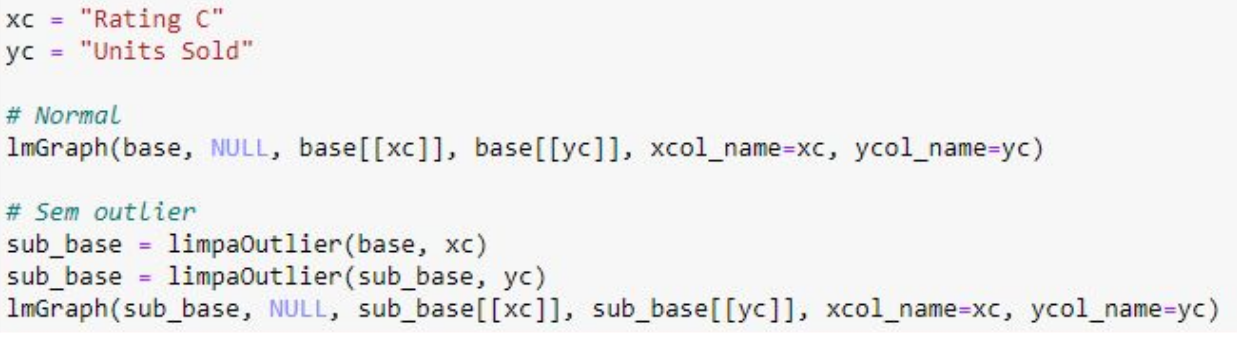
\includegraphics[scale=0.25, center]{./imgs/lm_us_rc.png}
\end{figure}
\FloatBarrier 

A figura a seguir (7) mostra o gŕafico de dispersão entre as variáveis Rating Count e Units Sold. Observa-se uma linearidade entre as variáveis, apesar do comportamento estranho da variável Units Sold, que possui os dados agrupados em valores específicos. Isso se deve ao fato de que, provavelmente, os valores dessa coluna foram arrendondados para faixas específicas de valores, o que causou a aparência atípica dos dados.

\FloatBarrier
\begin{figure}[h]
	\hspace{1cm}
  \begin{subfigure}[b]{0.4\textwidth}
    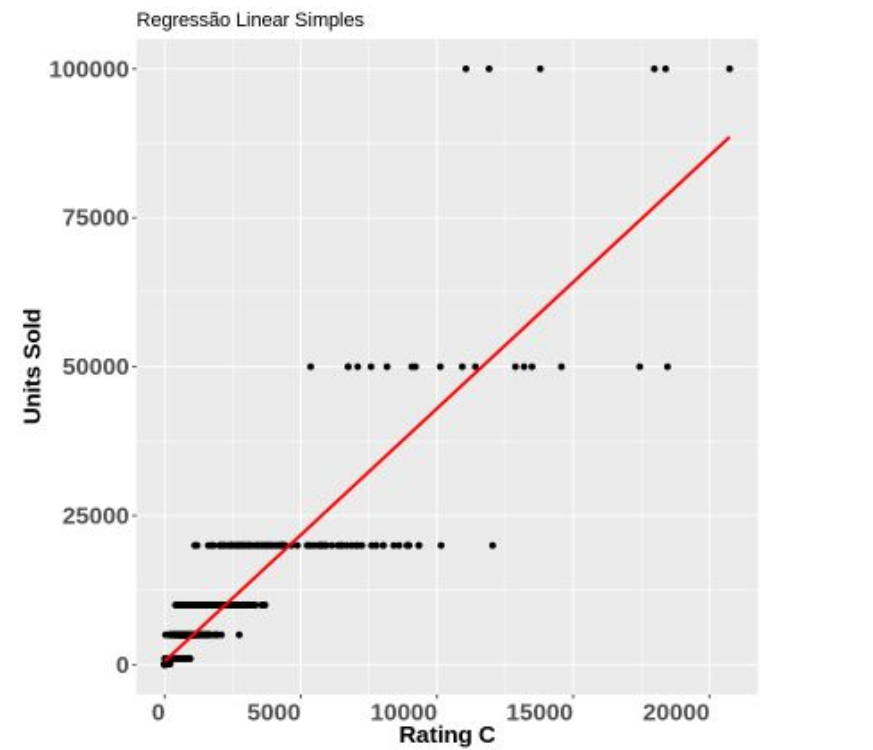
\includegraphics[scale=0.3, center]{./imgs/lm_us_rc_img.png}
    \caption*{7. Regressão Rating C e Units Sold}
    \label{fig:1}
  \end{subfigure}
  \hspace{0.25cm}
  \begin{subfigure}[b]{0.45\textwidth}
    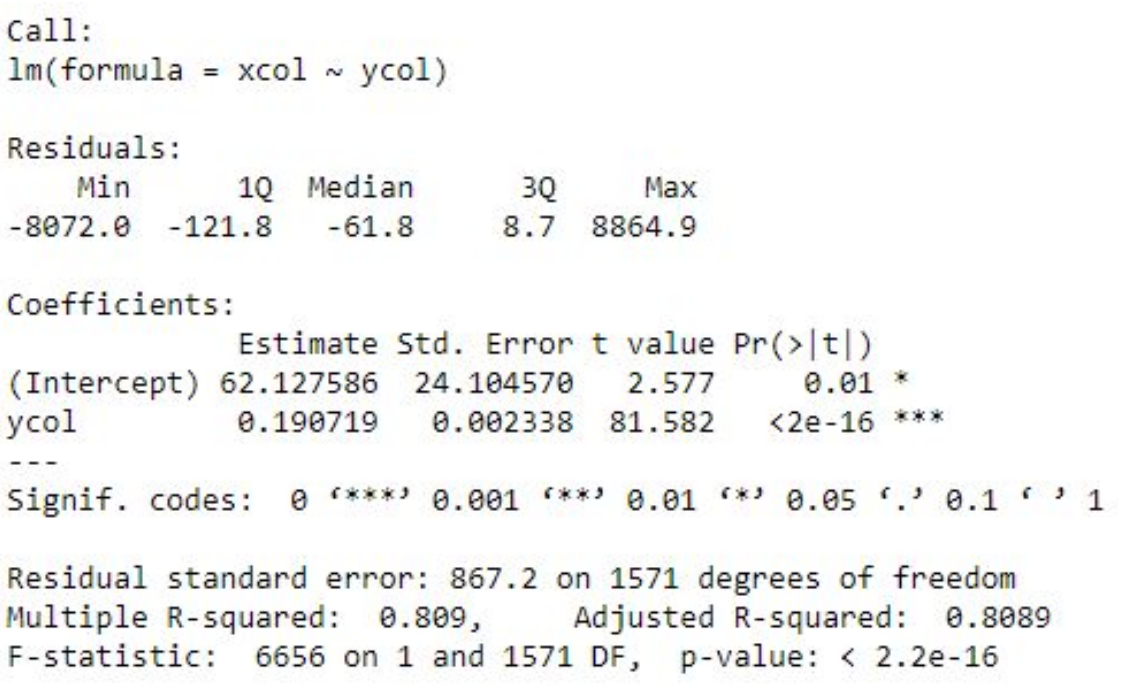
\includegraphics[scale=0.45, center]{./imgs/lm_us_rc_sum.png}
    \caption*{8. Sumário}
    \label{fig:2}
  \end{subfigure}
\end{figure}
\FloatBarrier

O mesmo procedimento de regressão linear foi executado , porém retirando os outliers das duas variáveis utilizadas. O resultado foi um $R^{2}$ muito menor, e um p-value muito alto, o que retira a significância estatística da variável. Isso foi feito pois os valores da parte superior da ordenada são pequenos em número porém algumas vezes maiores em magnetude que os valores na parte inferior.

\FloatBarrier
\begin{figure}[h]
	\hspace{1cm}
  \begin{subfigure}[b]{0.4\textwidth}
    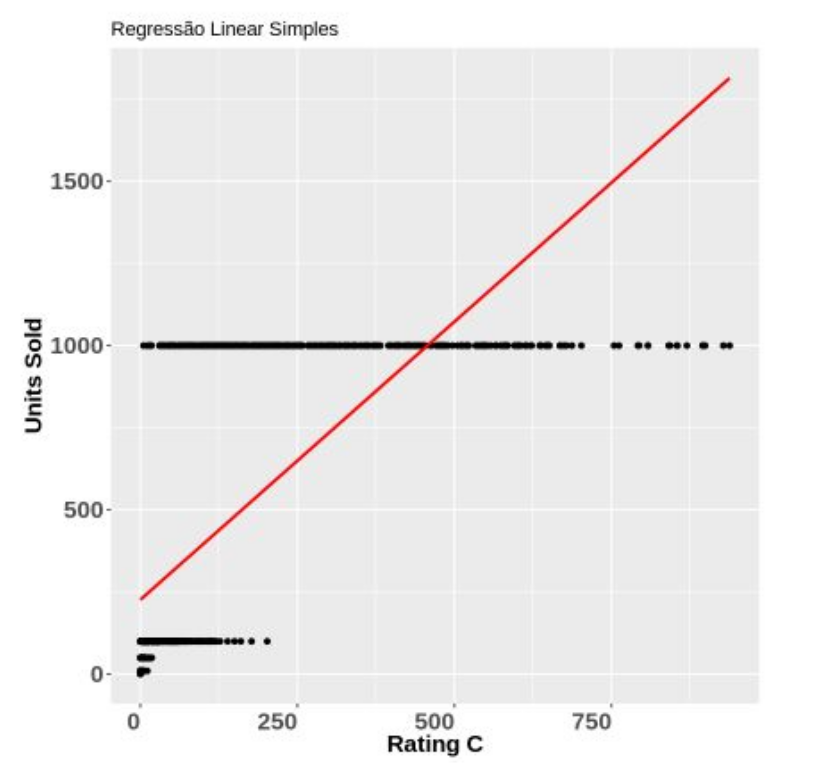
\includegraphics[scale=0.3, center]{./imgs/lm_us_rc_img_out.png}
    \caption*{9. Sem outliers}
    \label{fig:1}
  \end{subfigure}
  \hspace{0.5cm}
  \begin{subfigure}[b]{0.5\textwidth}
    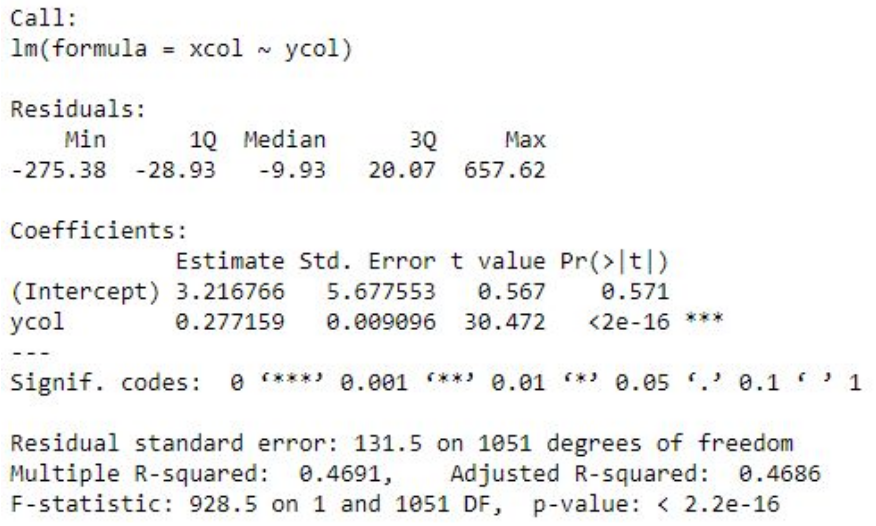
\includegraphics[scale=0.45, center]{./imgs/lm_us_rc_img_out_sum.png}
    \caption*{10. Sumário}
    \label{fig:2}
  \end{subfigure}
\end{figure}
\FloatBarrier

Veja que na segunda imagem (9) que sem aqueles valores o modelo centra-se no nas vendas feitas na linha de 1000 Units Sold que é bem larga e é desbalanceada de uma reta totalmente horizontal pelo grosso de valores na parte inferior. O fato da reta não passar mais pelo centro dos valores inferiores indica um desbalanceamente por falta dos valores superiores que ficavam mais a frente no eixo da abscissa.

Sobre os três pares do mapa de correlação foram feitas regressões, tanto antes quanto depois da remoção dos outliers, resultando em valores não satisfatórios. Houve aumento do valores de $R^{2}$, mas mesmo assim permaneceram abaixo de 0.2, porem o valor dos coeficientes lineares encotrados nos revelam algumas informações interessantes.

\FloatBarrier
\begin{figure}[h]
  \begin{subfigure}[b]{0.4\textwidth}
    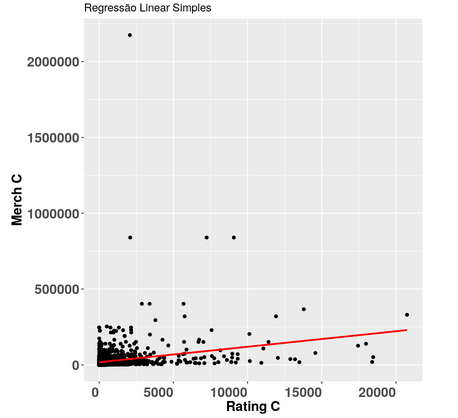
\includegraphics[scale=0.48, center]{./imgs/lm_mc_rc.png}
    \caption*{11. Merch C e Rating C}
    \label{fig:1}
  \end{subfigure}
  \begin{subfigure}[b]{0.5\textwidth}
    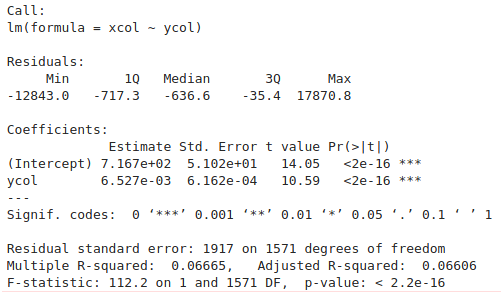
\includegraphics[scale=0.44, center]{./imgs/lm_mc_rc_s.png}
    \caption*{12. Sumário}
    \label{fig:2}
  \end{subfigure}
\end{figure}
\FloatBarrier 

\FloatBarrier
\begin{figure}[h]
  \begin{subfigure}[b]{0.4\textwidth}
    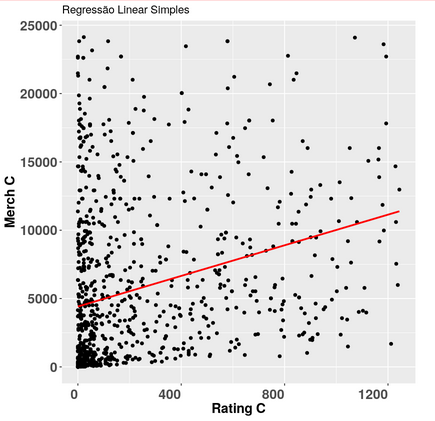
\includegraphics[scale=0.48, center]{./imgs/lm_mc_rc_o.png}
    \caption*{13. Sem outliers}
    \label{fig:1}
  \end{subfigure}
  \begin{subfigure}[b]{0.5\textwidth}
    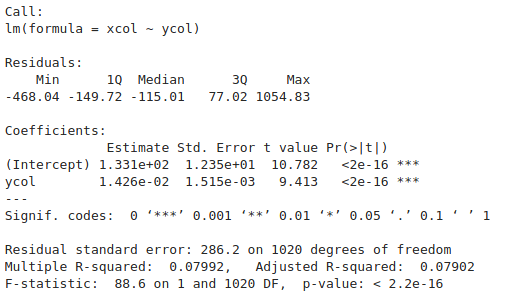
\includegraphics[scale=0.4, center]{./imgs/lm_mc_rc_o_s.png}
    \caption*{14. Sumário}
    \label{fig:2}
  \end{subfigure}
\end{figure}
\FloatBarrier 

\FloatBarrier
\begin{figure}[h]
  \hspace{1cm}
  \begin{subfigure}[b]{0.48\textwidth}
    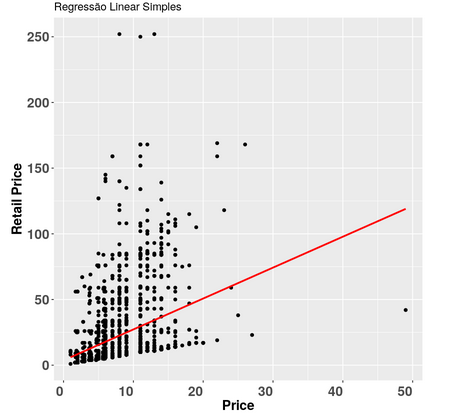
\includegraphics[scale=0.48, center]{./imgs/lm_rp_p.png}
    \caption*{15. Retail Price e Price}
    \label{fig:1}
  \end{subfigure}
  \begin{subfigure}[b]{0.5\textwidth}
    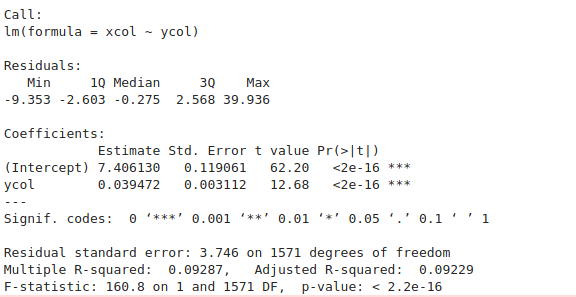
\includegraphics[scale=0.5, center]{./imgs/lm_rp_p_s.png}
    \caption*{16. Sumário}
    \label{fig:2}
  \end{subfigure}
\end{figure}
\FloatBarrier 

\FloatBarrier
\begin{figure}[h]
  \hspace{1.2cm}
  \begin{subfigure}[b]{0.4\textwidth}
    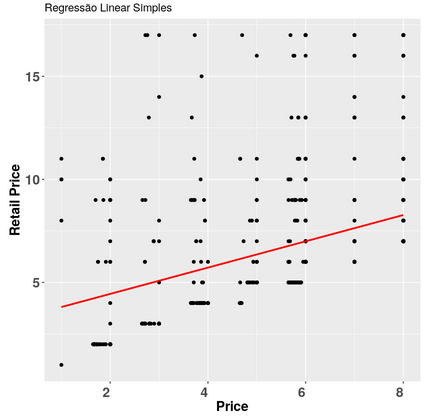
\includegraphics[scale=0.5, center]{./imgs/lm_rp_p_o.png}
    \caption*{17. Sem outliers}
    \label{fig:1}
  \end{subfigure}
    \hspace{0.4cm}
  \begin{subfigure}[b]{0.5\textwidth}
    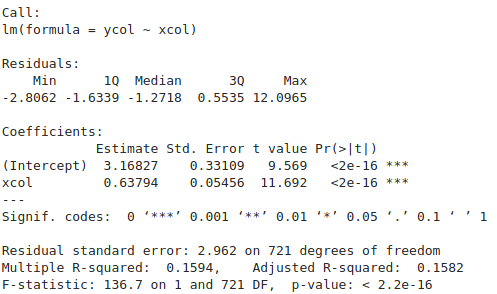
\includegraphics[scale=0.44, center]{./imgs/lm_rp_p_o_s.png}
    \caption*{18. Sumário}
    \label{fig:2}
  \end{subfigure}
\end{figure}
\FloatBarrier

Para essa regressão o valor original da tangente era de 2.3 que é maior do que 1, sendo assim os preços de varejo, ou seja os preços do consumidor final, tendem a subir quanto maiores forem os preços do item. Agora, na segunda análise esse valor cai ao se retirarem os preços altos de vende e revenda, com uma tangente de 0.63, quanto mais aumenta o preço do item, menos o consumdir final tende a pagar a mais por ele.

\FloatBarrier
\begin{figure}[h]
  \begin{subfigure}[b]{0.4\textwidth}
    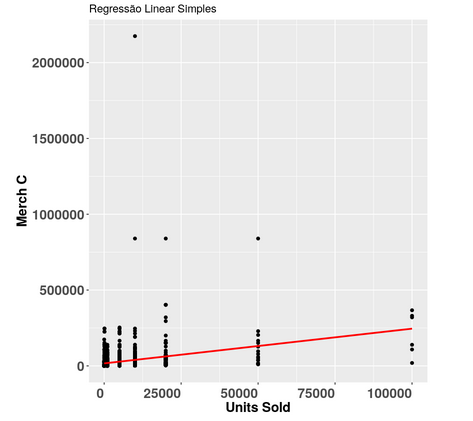
\includegraphics[scale=0.48, center]{./imgs/lm_mc_us.png}
    \caption*{19. Merch C e Units Sold}
    \label{fig:1}
  \end{subfigure}
  \begin{subfigure}[b]{0.5\textwidth}
    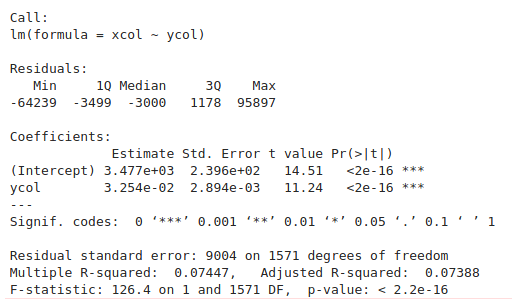
\includegraphics[scale=0.44, center]{./imgs/lm_mc_us_s.png}
    \caption*{20. Sumário}
    \label{fig:2}
  \end{subfigure}
\end{figure}
\FloatBarrier 

\FloatBarrier
\begin{figure}[h]
  \begin{subfigure}[b]{0.4\textwidth}
    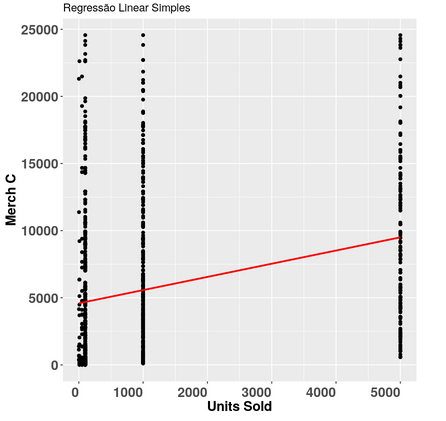
\includegraphics[scale=0.48, center]{./imgs/lm_mc_us_o.png}
    \caption*{21. Sem outliers}
    \label{fig:1}
  \end{subfigure}
  \begin{subfigure}[b]{0.5\textwidth}
    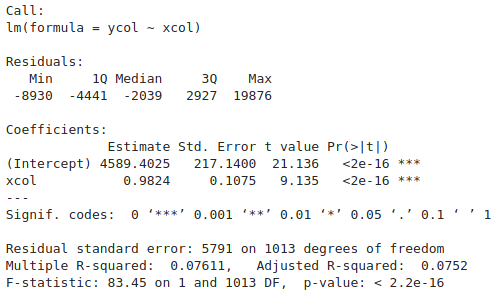
\includegraphics[scale=0.44, center]{./imgs/lm_mc_us_o_s.png}
    \caption*{22. Sumário}
    \label{fig:2}
  \end{subfigure}
\end{figure}
\FloatBarrier 

Foi feita uma regressão multipla com para Units Sold, que é uma variável de muito interesse, com todas as outras colunas exceto a Rating C que tem uma correlação muito alta. Os resultados também foram insatisfatórios, sem poder explicativo algum.

\FloatBarrier
\begin{figure}[h]
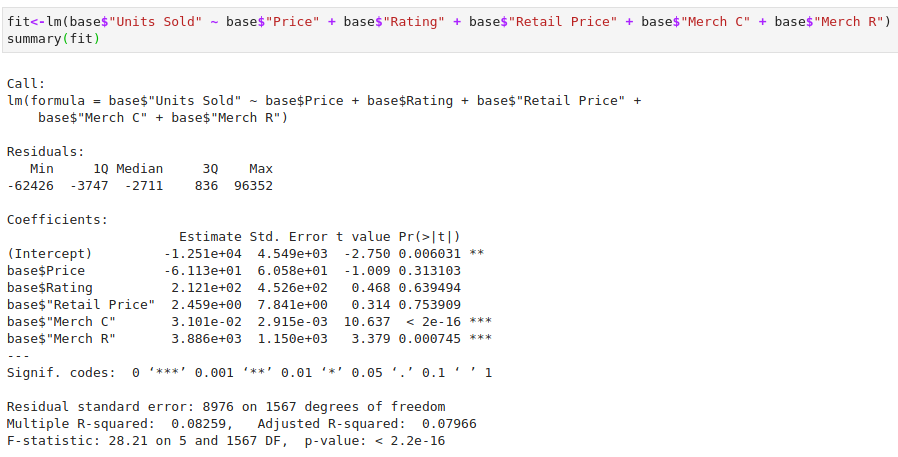
\includegraphics[scale=0.5, center]{./imgs/lmm_us.png}
\caption*{Figura 23: Regressão Multipla Units Sold}
\end{figure}
\FloatBarrier 

Por fim foram feitos o plot dos resíduos da regressão com outliers de Units Sold e Rating C, pelo Rating C e um histograma. A variância dos resíduos não é constante e aumenta tanto quanto aumenta Rating C, o que indica um modelo inadequado. O histograma aparenta ter uma distribuição normal dos resíduos. Um teste de Shapiro-Wilk revela os resultados de 0.55379 e o $p-value < 2.2e-16$, revelando que o modelo não é muito normal, assim rejeitamos a hipótse de normalidade.

\FloatBarrier
\begin{figure}[h]
  \begin{subfigure}[b]{0.4\textwidth}
    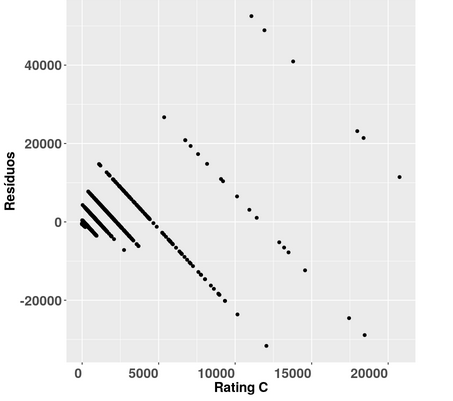
\includegraphics[scale=0.5, center]{./imgs/rs_rc_plot.png}
    \caption*{24. Resíduos e Rating C}
    \label{fig:1}
  \end{subfigure}
  \hspace{1.5cm}
  \begin{subfigure}[b]{0.5\textwidth}
    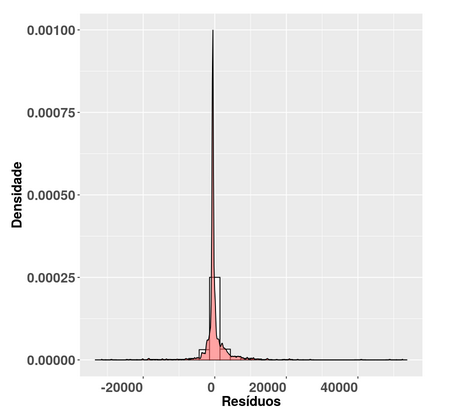
\includegraphics[scale=0.5, center]{./imgs/norm_rs_rc.png}
    \caption*{25. Histograma dos resíduos}
    \label{fig:2}
  \end{subfigure}
\end{figure}
\FloatBarrier 

\section{Referências}  
       
   	Sales of summer clothes in E-commerce Wish. \textbf{Kaggle}, 2020. Disponível em: $<$https://www.kaggle.\/\/com/jmmvutu/summer-products-and-sales-in-ecommerce-wish$>$.\\Acesso em: 3 de set. de 2020.
   	
   	HAIR, Joseph F. et al. Análise multivariada de dados. Bookman editora, 2009.
   	
	BUSSAB, Wilton O.; MORETTIN, Pedro A. Estatística Básica, 5ª Edição, São Paulo. Editora Saraiva, 2006.
	
	Sales of summer clothes in E-commerce Wish. \textbf{Kaggle}, 2020. Disponível em: $<$https://www.kaggle.\/\/com/jmmvutu/summer-products-and-sales-in-ecommerce-wish$>$.\\Acesso em: 3 de set. de 2020.
	
	Teste de Shapiro-Wilk. \textbf{Portal Action}. Disponível em: $<$    
    http://www.portalactio\\n.com.br/inferencia/64-teste-de-shapiro-wilk$/>$. Acesso em: 3 de set. de 2020.


\end{document}